\chapter{Teknologianalyse}\label{Teknologianalyse}

\section{Indledning til teknologianylse her}

\section{VisSim}
VisSim er et simulations program, som består af at man sætter blokke og diagrammer sammen, som former simuleringen. Det er en form for programmering, men man programmere ved brug af blokke og diagrammer. VisSim benyttes for general modellering, simulation og designe simulations applikationer. Programmet bruges til at konstruere og simulere større dynamiske systemer. VisSim er programmeret i ANSI C, og under processen af et VisSim projekt kan projektet kompileres.  
VisSim er et diskret simuleringsprogram som modellerer adfærden for den enkle billist. VisSim benytter sig af psyko fysisk model, som benytter en regelbaseret algoritme ved bevægelser på tværs af banerne. Den psykologiske del bliver brugt til bilistens ønske om aggressivitet, hastighed, reaktionsevne og generelt menneskelige forhold til trafikken. Den fysiske del bruges til bilens adfærd, så som bilens hastighed, størrelse, position. 

\subsection{VisSim - Bilen}
Den enkle bil spiller også en stor rolle hos VisSim, bilen er bestående af forskellige parametre, og det er ofte disse parametre der måles ved forsøg. Denne rapport tager udgangspunkt i acceleration og deceleration, ved vurdering af VisSim. Bilens parametre er beskrevet nedenfor.

\begin{itemize}
\item[Ønsket acceleration.]
\item[Deceleration.]
\item[Acceleration]
\item[Vægtfordeling.]
\item[Hastighedsfordeling.]
\item[Afstand mellem køretøjer.]
\item[Størrelsen på køretøjet.]
\end{itemize}

\subsection{VisSim - Netværket}
Netværket er bestående af de visuelle elementer, som har indflydelse på trafikafviklingen.
Netværket parametre er beskrevet nedenfor.

\begin{itemize}
\item[Rundkørsler.]
\item[Vigepligt.]
\item[Lyskryds(signalregulering).]
\item[Hastighedszone.]
\item[Vejbredde.]
\item[Vejlængde.]
\end{itemize}

\subsection{Analyse af acceleration og deceleration}
Ud fra en undersøgelse foretaget af Pihlkjær afgangsprojekt Aalborg Universitet - Vej og Trafikteknik, viser det sig at nogle af VisSims accelerations og decelerations værdier kan være upræcise. Undersøgelsen er foretaget ved analysering af VisSim på de danske vej-netværk.  Undersøgelsen bruger data fra vejdirektoratet, dette data sammenlignes med VisSims accelerations data.

På figur \ref{GrafForAccelerationVisSim}, kan man se at accelerations fordelingen for VisSim er markant højere end dataen fra Vejdirektoratet. Dette viser sig, at være pga. VisSim er henvendt til de tyske-vejnetværk. I undersøgelsen beskriver de, at det skyldes de tyske biler er større og hurtigere. Dog bruger rapporten ældre data fra Vejdirektoratet, og derfor kan undersøgelsen også vise sig at være upræcis.

\begin{figure}
\begin{center}
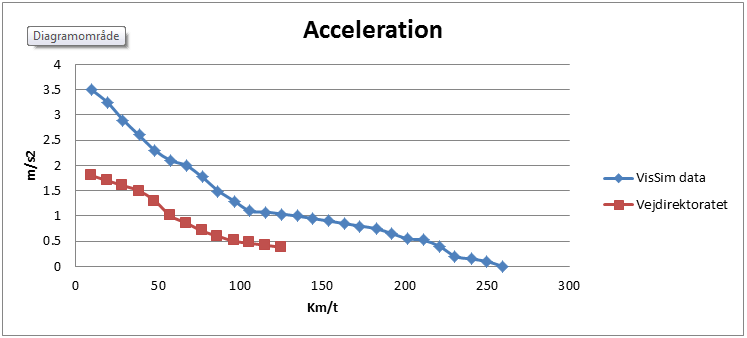
\includegraphics[width=1.0\textwidth]{Pictures/Teknologianalyse/GrafForAccelerationVisSim.png}
\end{center}
\label{GrafForAccelerationVisSim}
\caption{graf}
\end{figure}

Der er yderlige undersøgelser foretaget af Pihlkjær afgangsprojekt Aalborg Universitet - Vej og Trafikteknik, hvor der sammenlignes med GPS accelerations og decleration data, med VisSims data. Her er der blevet indsat GPS i 166 bilister som skal repræsentere acceleration og deceleration i Danmark. På figur \ref{GrafForAccelerationVisSimGPS} kan man se, at det stadigvæk viser sig at VisSims acceleration er markant højere, end GPS daten. Dette kan give upræcis data, ved brug af simulering. 

\begin{figure}
\begin{center}
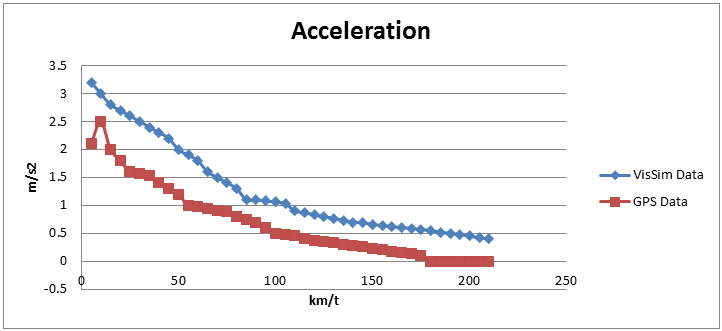
\includegraphics[width=1.0\textwidth]{Pictures/Teknologianalyse/GrafForAccelerationVisSimGPS.png}
\end{center}
\label{GrafForAccelerationVisSimGPS}
\caption{graf}
\end{figure}

Samtidig er der undersøgt af Pihlkjær afgangsprojekt Aalborg Universitet - Vej og Trafikteknik om deceleration for bilister er præcise i VisSim, dette er også gjort ved sammenligning af VisSim data, med GPS data. På figur \ref{GrafForDecelerationVisSimGPS} kan man se, at VisSims deceleration er markant højere end GPS dataen, man ser også at VisSim er lineæret udspillet. Det vurderes at dette kan have betydning for udfaldet i simleringen, hvis VisSims data var nær GPS daten, så ville udfaldet blive mere præcist. Man ser også at VisSims data er konstant dette betyder, at programmet ikke variere decelerationen, i forhold til farten. 

\begin{figure}
\begin{center}
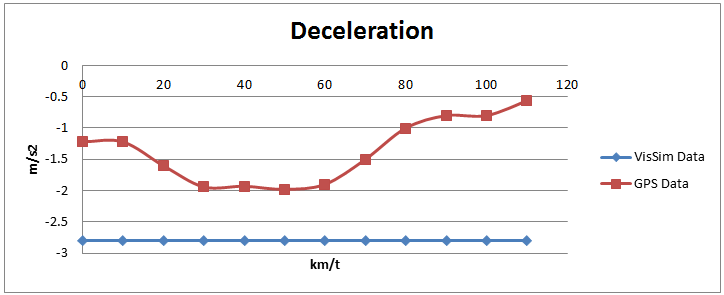
\includegraphics[width=1.0\textwidth]{Pictures/Teknologianalyse/GrafForDecelerationVisSimGPS.png}
\end{center}
\label{GrafForDecelerationVisSimGPS}
\caption{graf}
\end{figure}

